% Sandia National Laboratories is a multimission laboratory managed and
% operated by National Technology & Engineering Solutions of Sandia, LLC, a
% wholly owned subsidiary of Honeywell International Inc., for the U.S.
% Department of Energy’s National Nuclear Security Administration under
% contract DE-NA0003525.

% Copyright 2002-2021 National Technology & Engineering Solutions of Sandia,
% LLC (NTESS).


%%-------------------------------------------------------------------------
%% Purpose        : Main LaTeX Xyce Reference Guide
%% Special Notes  : Graphic files (pdf format) work with pdflatex.  To use
%%                  LaTeX, we need to use postcript versions.
%% Creator        : Eric R. Keiter, Computational Sciences, SNL
%% Creation Date  : {01/26/2003}
%%
%%-------------------------------------------------------------------------

%%
%% PDE Device simulation/TCAD Device Simulation.
%%
\clearpage
\section{TCAD Devices}
\index{device!PDE Devices}\index{PDE Devices}\index{TCAD Devices}
% Sandia National Laboratories is a multimission laboratory managed and
% operated by National Technology & Engineering Solutions of Sandia, LLC, a
% wholly owned subsidiary of Honeywell International Inc., for the U.S.
% Department of Energy’s National Nuclear Security Administration under
% contract DE-NA0003525.

% Copyright 2002-2020 National Technology & Engineering Solutions of Sandia,
% LLC (NTESS).


Semiconductor device simulation, which is based on a coupled set of partial
differential equations (PDE's) is supported in \Xyce{}.  Such devices can be
invoked from the circuit netlist in a manner similar to traditional SPICE-style
analog devices.  One dimensional and two dimensional devices are supported,
with the dimensionality determined by the device model level.

\begin{Device}

\item[1D Device Form]
\begin{alltt}
YPDE <name> <node> [node] [model name]
+ [device parameters]
\end{alltt}

\vbox{\hrulefill}
\item[2D Device Form]
\begin{alltt}
YPDE <name> <node> <node> [node][node] [model name]|
+ [device parameters]
\end{alltt}

\model
\begin{alltt}
.MODEL <model name> ZOD [model parameters]
\end{alltt}

\comments

All of the PDE parameters are specified on the instance level.  The model
statement is used only for specifying if the device is 1D or 2D, via the level
parameter.  Both the 1D and the 2D devices can construct evenly-spaced meshes
internally, or an unstructured mesh can be read in from an external mesh file.

The eletrode, doping and material parameters are specified using a special
format that is described in the tables that are referenced in the instance
parameter tables.
\end{Device}

\paragraph{TCAD Device Parameters}
Most TCAD device parameters are specified on the instance level.
\noindent
The only TCAD device model parameter is the level, which specifies whether the
model is one or two dimensions.

\label{PDE_Model_Params}
\index{PDE Devices!model parameters}
\begin{DeviceParamTable}{PDE Device Model Parameters}
LEVEL & Determines if the device is 1D or 2D  1=1D, 2=2D & -- & 1 \\ \hline
\end{DeviceParamTable}

\index{PDE Devices!1D instance parameters}
% This table was generated by Xyce:
%   Xyce -doc_cat Pde 1
%
\index{1d pde (level 1)!device instance parameters}
\begin{DeviceParamTableGenerated}{1D PDE (level 1) Device Instance Parameters}{Pde_1_Device_Instance_Params}
AUGER & Flag to turn on/off Auger recombination & logical (T/F) & true \\ \hline
BULKMATERIAL & Bulk semiconductor material & -- & 'SI' \\ \hline
DOPINGPROFILES &  & \multicolumn{2}{c}{See Table~\ref{DOPINGPROFILES_Composite_Params}}  \\ \hline
FERMIDIRAC & Use Fermi-Dirac statistics. & logical (T/F) & false \\ \hline
FIELDDEP & If true, use field dependent mobility. & logical (T/F) & false \\ \hline
LAYER &  & \multicolumn{2}{c}{See Table~\ref{LAYER_Composite_Params}}  \\ \hline
MASKVARSTIA & If set to true, then some variables are excluded from the time integration error control calculation. & logical (T/F) & false \\ \hline
MAXVOLTDELTA & Maximum voltage change used by two-level Newton algorithm. & V & 0.025 \\ \hline
MESHFILE &  & -- & 'internal.msh' \\ \hline
MOBMODEL & Mobility model. & -- & 'ARORA' \\ \hline
NODE &  & \multicolumn{2}{c}{See Table~\ref{NODE_Composite_Params}}  \\ \hline
NX & Number of mesh points & -- & 11 \\ \hline
REGION &  & \multicolumn{2}{c}{See Table~\ref{REGION_Composite_Params}}  \\ \hline
SRH & Flag to turn on/off Shockley-Read-Hall (SRH) recombination. & logical (T/F) & true \\ \hline
THERMIONICEMISSION &  & logical (T/F) & false \\ \hline
TUNNELING &  & -- & 'none' \\ \hline
USEOLDNI & Flag for using old(inaccurate) intrinsic carrier calculation. & logical (T/F) & false \\ \hline
VOLTLIM & Flag to apply voltage limiting.  This is only relevant for an experimental two-level Newton solver. & logical (T/F) & false \\ \hline

\category{Doping Parameters}\\ \hline
DOPING\_FILE & File containing doping profile. & -- & 'NOFILE' \\ \hline
GRADED & Flag for graded junction vs. abrupt junction. – (1/true=graded, 0/false=abrupt) & logical (T/F) & false \\ \hline
NA & Acceptor doping level & cm$^{-3}$ & 1e+15 \\ \hline
ND & Donor doping level & cm$^{-3}$ & 1e+15 \\ \hline
NDOPE\_FILE & File containing doping profile for N-type dopants. & -- & 'NOFILE' \\ \hline
PDOPE\_FILE & File containing doping profile for P-type dopants. & -- & 'NOFILE' \\ \hline
WJ & Junction width, if graded junction enabled. & cm & 0.0001 \\ \hline

\category{Geometry Parameters}\\ \hline
ANODE.AREA & Anode area (used for two-terminal devices) & cm$^{-2}$ & 0 \\ \hline
AREA & Cross sectional area of the device. & cm$^{-2}$ & 1 \\ \hline
BASE.AREA & Base area (used for three-terminal (BJT) devices) & cm$^{-2}$ & 0 \\ \hline
BASE.LOC & Location of base contact (necessary if running with three terminals). & cm & 0.0005 \\ \hline
CATHODE.AREA & Cathode area (used for two-terminal devices) & cm$^{-2}$ & 0 \\ \hline
COLLECTOR.AREA & Collector area (used for three-terminal (BJT) devices) & cm$^{-2}$ & 0 \\ \hline
EMITTER.AREA & Emitter area (used for three-terminal (BJT) devices) & cm$^{-2}$ & 0 \\ \hline
L & Device width. (Synonym with W parameter) & cm & 0.001 \\ \hline
W & Device width. (Synonym with L parameter) & cm & 0.001 \\ \hline

\category{Temperature Parameters}\\ \hline
TEMP & Device temperature & $^\circ$C & 27 \\ \hline

\category{Model Output Parameters}\\ \hline
FIRSTELECTRODEOFFSET & This is an output parameter.  It is only used if OFFSETOUTPUTVOLTAGE=true. (see description of that paramaeter & logical (T/F) & false \\ \hline
GNUPLOTLEVEL & Flag for gnuplot output.
0 - no gnuplot files.
1 - gnuplot files.
gnuplot is an open source plotting program that is usually installed on Linux systems. gnuplot files will have the *Gnu.dat suffix, and the prefix will be thename of the device instance. & -- & 1 \\ \hline
OFFSETOUTPUTVOLTAGE & This is an output parameter that determines the ``zero'' of the potential at output.  If OFFSETOUTPUTVOLTAGE=true (default) it will adjust the voltages at output so that the minimum voltage is zero. If true and also FIRSTELECTRODEOFFSET=true, then the voltage of the first electrode is the zero point.  If OFFSETOUTPUTVOLTAGE=false, the output voltage sets the intrisic Fermi level to zero.  Depending on circumstances each of these may be more or less convenient for plotting. & logical (T/F) & true \\ \hline
OUTPUTINTERVAL & Time interval for tecplot output (if tecplot is enabled). & s & 0 \\ \hline
OUTPUTNLPOISSON & Flag to determine if the results of the nonlinear Poisson calculation is included in the output files.  Normally, this calculation is used to initialize a drift-diffusion calculation and isn't of interest. & logical (T/F) & false \\ \hline
%SGPLOTLEVEL & Flag for sgplot output.
%0 - no sgplot files.
%1 - sgplot files.
%sgplot is a plotting program that comes as part of the SG Framework. sgplot files will have the *.res suffix, and the prefix will be the name of the device instance & -- & 0 \\ \hline
TECPLOTLEVEL & Setting for Tecplot output:
0 - no Tecplot files
1 - Tecplot files, each output in a separate file. 2 - Tecplot file, each outputappended to a single file.
Tecplot files will have the .dat suffix, and the prefix will be the name of the device instance & -- & 1 \\ \hline

\category{Scaling Parameters}\\ \hline
C0 & Density scalar; adjust to mitigate convergence problems.The model will do all of its scaling automatically, so it is generally not necessary to specify it manually. & cm$^{-3}$ & 1e+15 \\ \hline
DENSITYSCALARFRACTION & Fraction of the maximum doping by which density will be scaled.The model will do all of its scaling automatically, so it is generally not necessary to specify it manually. & logical (T/F) & 0.1 \\ \hline
SCALEDENSITYTOMAXDOPING & If set the density will be scaled by a fraction of the maximum doping.The model will do all of its scaling automatically, so it is generally not necessary to specify it manually. & logical (T/F) & true \\ \hline
t0 & Time scalar; adjust to mitigate convergence problems.The model will do all of its scaling automatically, so it is generally not necessary to specify it manually. & s & 1e-06 \\ \hline
X0 & Length scalar; adjust to mitigate convergence problems.The model will do all of its scaling automatically, so it is generally not necessary to specify it manually. & cm & 1e-07 \\ \hline

\category{Boundary Condition Parameters}\\ \hline
ANODE.BC & Anode voltage boundary condition.  Only used if device is uncoupled from circuit, and running in diode mode.
 & V & 0.5 \\ \hline
BASE.BC & Base voltage boundary condition.  Only used if device is uncoupled from circuit, and running in BJT mode.
 & V & 0 \\ \hline
CATHODE.BC & Cathode voltage boundary condition.  Only used if device is uncoupled from circuit, and running in diode mode.
 & V & 0 \\ \hline
COLLECTOR.BC & Collector voltage boundary condition.  Only used if device is uncoupled from circuit, and running in BJT mode.
 & V & 0 \\ \hline
EMITTER.BC & Emitter voltage boundary condition.  Only used if device is uncoupled from circuit, and running in BJT mode.
 & V & 0.5 \\ \hline
\end{DeviceParamTableGenerated}

\clearpage

\index{PDE Devices!1D instance parameters}
% This table was generated by Xyce:
%   Xyce -doc_cat Pde 2
%
\index{2d pde (level 2)!device instance parameters}
\begin{DeviceParamTableGenerated}{2D PDE (level 2) Device Instance Parameters}{Pde_2_Device_Instance_Params}
BULKMATERIAL & Material of bulk material. & -- & 'SI' \\ \hline
DISPLCUR & If true, displacement current is computed and output & logical (T/F) & false \\ \hline
DOPINGPROFILES &  & \multicolumn{2}{c}{See Table~\ref{DOPINGPROFILES_Composite_Params}}  \\ \hline
MAXVOLTDELTA & Maximum voltage change used by two-level Newton algorithm. & V & 0.025 \\ \hline
MESHFILE & This is a required field for a 2D simulation.  If the userspecifies meshfile=internal.mesh, the model will create aCartesian mesh using the parameters L,W,NX and NY.  If the user specifies anything else (for example meshfile=diode.msh), the model will attempt to read in a mesh file of that name.  The format is assumed to be that of the SG Framework. & -- & 'internal.msh' \\ \hline
MOBMODEL & Mobility model. & -- & 'ARORA' \\ \hline
NODE &  & \multicolumn{2}{c}{See Table~\ref{NODE_2D_Composite_Params}}  \\ \hline
NX & Number of mesh points, x-direction. & -- & 11 \\ \hline
NY & Number of mesh points, y-direction. & -- & 11 \\ \hline
REGION &  & \multicolumn{2}{c}{See Table~\ref{REGION_Composite_Params}}  \\ \hline
TYPE & P-type or N-type - this is only relevant if using the default dopings & -- & 'PNP' \\ \hline
USEMATRIXGID &  & -- & false \\ \hline
USEOLDNI & Flag for using old (inaccurate) intrinsic carrier calculation. & logical (T/F) & false \\ \hline
USEVECTORGID &  & -- & false \\ \hline
VOLTLIM &  & logical (T/F) & false \\ \hline

\category{Doping Parameters}\\ \hline
GRADED & Flag for graded junction vs. abrupt junction. – (1/true=graded, 0/false=abrupt) & logical (T/F) & false \\ \hline
NA & Acceptor doping level & cm$^{-3}$ & 1e+15 \\ \hline
ND & Donor doping level & cm$^{-3}$ & 1e+15 \\ \hline
WJ & Junction width, if graded junction enabled. & cm & 0.0001 \\ \hline

\category{Geometry Parameters}\\ \hline
AREA & Cross sectional area of the device. & cm$^{-2}$ & 1 \\ \hline
CYL & Flag to enable cylindrical geometry & logical (T/F) & false \\ \hline
L & Device length & cm & 0.001 \\ \hline
W & Device width & cm & 0.001 \\ \hline

\category{Temperature Parameters}\\ \hline
TEMP & Device temperature & $^\circ$C & 27 \\ \hline

\category{Model Output Parameters}\\ \hline
GNUPLOTLEVEL & Flag for gnuplot output.
0 - no gnuplot files.
1 - gnuplot files.
gnuplot is an open source plotting program that is usually installed on Linux systems. gnuplot files will have the *Gnu.dat suffix, and the prefix will be thename of the device instance. & -- & 0 \\ \hline
INTERPGRIDSIZE &  & -- & 20 \\ \hline
OUTPUTINTERVAL & Time interval for tecplot output (if tecplot is enabled). & s & 0 \\ \hline
OUTPUTNLPOISSON & Flag to determine if the results of the nonlinear Poisson calculation is included in the output files.  Normally, this calculation is used to initialize a drift-diffusion calculation and isn't of interest. & logical (T/F) & false \\ \hline
%SGPLOTLEVEL & Flag for sgplot output.
%0 - no sgplot files.
%1 - sgplot files.
%sgplot is a plotting program that comes as part of the SG Framework. sgplot files will have the *.res suffix, and the prefix will be the name of the device instance & -- & 0 \\ \hline
TECPLOTLEVEL & Setting for Tecplot output:
0 - no Tecplot files
1 - Tecplot files, each output in a separate file. 2 - Tecplot file, each outputappended to a single file.
Tecplot files will have the .dat suffix, and the prefix will be the name of the device instance & -- & 1 \\ \hline
TXTDATALEVEL & Flag for volume-averaged text output.
0 - no text files.
1 - text files.
txtdataplot files will have the *.txt suffix, and the prefix will be the name of the device instance. & -- & 1 \\ \hline

\category{Scaling Parameters}\\ \hline
X0 & Length scalar; adjust to mitigate convergence problems. The model will do all of its scaling automatically, so it is generally not necessary to specify it manually. & cm & 0.0001 \\ \hline

\category{Boundary Condition Parameters}\\ \hline
CONSTBOUNDARY &  & -- & false \\ \hline
\end{DeviceParamTableGenerated}

\clearpage

\paragraph{Layer Parameters}
% This table was generated by Xyce
\index{layer!composite parameters}
\begin{CompositeParamTableGenerated}{LAYER Composite Parameters}{LAYER_Composite_Params}
CON &  & -- & 1.42248 \\ \hline
ConductionBandDOS &  & -- & 2.89e+19 \\ \hline
DIEL &  & -- & 13.1 \\ \hline
ELMOB0 &  & -- & 2240 \\ \hline
ELVSAT &  & -- & 7.7e+06 \\ \hline
EMASS &  & -- & 0.067 \\ \hline
GRADEDWIDTH &  & -- & 0 \\ \hline
HMASS &  & -- & 0.5 \\ \hline
HOMOB0 &  & -- & 30 \\ \hline
HOVSAT &  & -- & 7.7e+06 \\ \hline
MATERIAL &  & -- & 'gaas' \\ \hline
NAME &  & -- & 'EMITTER' \\ \hline
NARCO &  & -- & 0.047 \\ \hline
NARVA &  & -- & 0.047 \\ \hline
NDOPE &  & -- & 0 \\ \hline
NI &  & -- & 1.79e+06 \\ \hline
NX &  & -- & 25 \\ \hline
PDOPE &  & -- & 5e+19 \\ \hline
VAL &  & -- & 0 \\ \hline
ValenceBandDOS &  & -- & 2.66e+19 \\ \hline
WIDTH &  & -- & 1e-06 \\ \hline
\end{CompositeParamTableGenerated}


\paragraph{Electrode Parameters 1D}
% This table was generated by Xyce
\index{node!composite parameters}
\begin{CompositeParamTableGenerated}{NODE Composite Parameters}{NODE_Composite_Params}
AREA &  & -- & 0 \\ \hline
BC & Carrier density boundary condition type (dirichlet or neumann) & -- & 'dirichlet' \\ \hline
LOCATION &  & -- & 0 \\ \hline
MATERIAL & Contact material & -- & 'neutral' \\ \hline
NAME & Electrode name & -- & 'anode' \\ \hline
OXIDEBNDRYFLAG & Oxide layer boolean & -- & false \\ \hline
SIDE & Side specification (left or right) & -- & 'left' \\ \hline
\end{CompositeParamTableGenerated}


\paragraph{Electrode Parameters 2D}
% This table was generated by Xyce
\index{node!composite parameters}
\begin{CompositeParamTableGenerated}{NODE Composite Parameters}{NODE_2D_Composite_Params}
BC & Carrier density boundary condition type (dirichlet or neumann) & -- & 'dirichlet' \\ \hline
END & Ending location & cm & 0 \\ \hline
MATERIAL & Contact material & -- & 'neutral' \\ \hline
NAME & Electrode name & -- & 'anode' \\ \hline
OXCHARGE & Oxide charge & -- & 0 \\ \hline
OXIDEBNDRYFLAG & Oxide layer boolean & -- & false \\ \hline
OXTHICK & Oxide thickness & cm & 0 \\ \hline
SIDE & Side specification (top, bottom, left or right) & -- & 'top' \\ \hline
START & Starting location & cm & 0 \\ \hline
\end{CompositeParamTableGenerated}


\paragraph{Doping or Region Parameters}
The \texttt{DOPINGPROFILES} and \texttt{REGION} parameters are synonyms,
therefore their tables of values are identical.  The use of both parameters in
the same device instance could lead to unpredictable behavior.
% This table was generated by Xyce
\index{dopingprofiles!composite parameters}
\begin{CompositeParamTableGenerated}{DOPINGPROFILES Composite Parameters}{DOPINGPROFILES_Composite_Params}
EL2 &  & -- & 0 \\ \hline
EXPRESSION & User-defined expressions for dopant profiles as function of depth  & -- & 'none' \\ \hline
FILE &  & -- & 'none' \\ \hline
FLATX & Determines the doping shape (half-gaussian or a full gaussian) & -- & 0 \\ \hline
FLATY & 2D ONLY: Determines the doping shape (half-gaussian or a full gaussian) & -- & 0 \\ \hline
FUNCTION & Functional form of doping region; options are uniform, gaussian, and step. & -- & 'uniform' \\ \hline
NAME &  & -- & 'none' \\ \hline
NMAX & Maximum value of impurity concentration & cm$^{-3}$ & 1e+15 \\ \hline
NMAXCHOP &  & cm$^{-3}$ & 1e+20 \\ \hline
NMIN & Minimum value of impurity concentration & cm$^{-3}$ & 0 \\ \hline
SPECIES &  & -- & 'none' \\ \hline
TYPE & ntype or ptype & -- & 'ntype' \\ \hline
XLOC & Peak location of the doping in the x-direction & cm & 0 \\ \hline
XMAX &  & cm & 0 \\ \hline
XMIN &  & cm & 0 \\ \hline
XWIDTH & Distance from nmax to nmin. This is only applicable for the function=gaussian case. & cm & 0.001 \\ \hline
YLOC & 2D ONLY: Peak location of the doping in the y-direction () & cm & 0 \\ \hline
YMAX & 2D ONLY:  & cm & 0 \\ \hline
YMIN & 2D ONLY:  & cm & 0 \\ \hline
YWIDTH & 2D ONLY: Distance from nmax to nmin. This is only applicable for the function=gaussian case. & cm & 0.001 \\ \hline
\end{CompositeParamTableGenerated}

% This table was generated by Xyce
\index{region!composite parameters}
\begin{CompositeParamTableGenerated}{REGION Composite Parameters}{REGION_Composite_Params}
EL2 &  & -- & 0 \\ \hline
EXPRESSION &  & -- & 'none' \\ \hline
FILE &  & -- & 'none' \\ \hline
FLATX & Determines the doping shape (half-gaussian or a full gaussian) & -- & 0 \\ \hline
FLATY & 2D ONLY: Determines the doping shape (half-gaussian or a full gaussian) & -- & 0 \\ \hline
FUNCTION & Functional form of doping region; options are uniform, gaussian, and step. & -- & 'uniform' \\ \hline
NAME &  & -- & 'none' \\ \hline
NMAX & Maximum value of impurity concentration & cm$^{-3}$ & 1e+15 \\ \hline
NMAXCHOP &  & cm$^{-3}$ & 1e+20 \\ \hline
NMIN & Minimum value of impurity concentration & cm$^{-3}$ & 0 \\ \hline
SPECIES &  & -- & 'none' \\ \hline
TYPE & ntype or ptype & -- & 'ntype' \\ \hline
XLOC & Peak location of the doping in the x-direction & cm & 0 \\ \hline
XMAX &  & cm & 0 \\ \hline
XMIN &  & cm & 0 \\ \hline
XWIDTH & Distance from nmax to nmin. This is only applicable for the function=gaussian case. & cm & 0.001 \\ \hline
YLOC & 2D ONLY: Peak location of the doping in the y-direction () & cm & 0 \\ \hline
YMAX & 2D ONLY:  & cm & 0 \\ \hline
YMIN & 2D ONLY:  & cm & 0 \\ \hline
YWIDTH & 2D ONLY: Distance from nmax to nmin. This is only applicable for the function=gaussian case. & cm & 0.001 \\ \hline
\end{CompositeParamTableGenerated}


\paragraph{Flat Parameters}
% Sandia National Laboratories is a multimission laboratory managed and
% operated by National Technology & Engineering Solutions of Sandia, LLC, a
% wholly owned subsidiary of Honeywell International Inc., for the U.S.
% Department of Energy’s National Nuclear Security Administration under
% contract DE-NA0003525.

% Copyright 2002-2021 National Technology & Engineering Solutions of Sandia,
% LLC (NTESS).


%%
%% Table describing the flatx, flaty parameters.
%%

\newenvironment{FlatTable}[1]
               {\renewcommand{\arraystretch}{1.5}
                 \newcommand{\category}[1]{\multicolumn{4}{c}{\smallskip\color{XyceDarkBlue}\em\bfseries ##1}}
                 \begin{longtable}{>{\ttfamily\small}m{1in}<{\normalfont}>{\raggedright\small}m{3in}>{\raggedright\let\\\tabularnewline\small}m{1in}}
                   \caption{#1} \\ \hline}
               {\end{longtable}}

%% ERK: Note:  I made each row of the table actually be two rows, because the 
%% graphical cross section picture, which is coming from a jpg file, was 
%% tending to overwrite the lines of the table.  In particular, it was 
%% overwriting the line immediately above it.  It did this for every 
%% (length, width) value that I tried.
%%
\begin{FlatTable}{Description of the flatx, flaty doping parameters\label{flatxy_table}}
    \rowcolor{XyceDarkBlue}
    \color{white}\normalfont\bf Flatx or Flaty view  &
    \color{white}\bf Description &
    \color{white}\bf 1D Cross Section \endhead

   0  & Gaussian on both sides of the peak (\texttt{xloc}) location. & {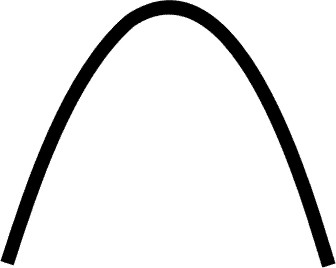
\includegraphics[width=0.300in,height= 0.300in]{flatxy1}} \\ \hline
  +1  & Gaussian if \texttt{x>xloc}, flat (constant at the peak value) if \texttt{x<xloc}. & {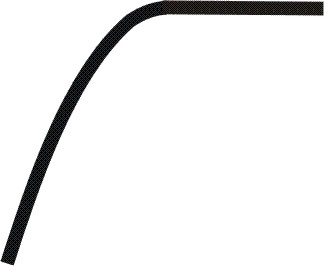
\includegraphics[width=0.300in,height= 0.300in]{flatxy2}} \\ \hline
  -1  & Gaussian if \texttt{x<xloc}, flat (constant at the peak value) if \texttt{x>xloc}. & {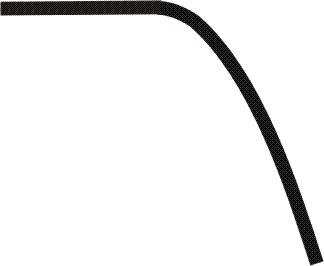
\includegraphics[width=0.300in,height= 0.300in]{flatxy3}} \\ \hline
\end{FlatTable}





\newpage
\subsection{Physical Models}
\index{PDE Devices!Physical Models}
\index{TCAD Devices!Physical Models}

This section contains information about physical models used in \Xyce{}
for TCAD devices.  This includes various mobility models, expressions
for calculating the effective mass for electrons and holes, an expression
for intrinsic carrier concentration as a function of temperature,
expressions which describe contacts to metal as well as contacts to
metal-oxide-semiconductor devices.

\subsubsection{Material Models and Parameters}
\label{material}

This section describes some of the basic material properties that are 
available in \Xyce{}.  Described here are the models for effective mass,
intrinsic carrier concentration, and the bandgap.  This information is needed
for the more complex models described in the mobility section
(section~\ref{mobility}) and the boundary condition section
(section~\ref{boundaryCondition}).

\subsubsection{Effective Mass}
\Xyce{} includes functions which return the effective mass of electrons and
holes for a number of semiconductor materials.

\subsubsection{Electron Effective Mass}
The electron effective mass is calculated as

\begin{equation}
 m_{de} = (m_{l}^{*} m_{t}^{*2})^{1/3}
\end{equation}

where $m_{l}$ and $m_{t}$ are the effective masses along the longitudinal
and transverse directions of the ellipsoidal energy surface.

\subsubsection{Hole Effective Mass}
The hole effective mass is calculated as
\begin{equation}
  m_{dh} = (m_{lh}^{*3/2} + m_{hh}^{*3/2})^{2/3}
\end{equation}

where $m_{lh}$ and $m_{hh}$ are the "light" and "heavy" hole masses,
respectively.

\subsubsection{Intrinsic Carrier Concentration}

The intrinsic carrier concentration in a semiconductor is obtained from the
"np" product

\begin{equation}
  np = n_{i}^{2} = N_{C}N_{V} exp(-E_{g}/kT)
\end{equation}

or
\begin{equation}
 n_{i} = \sqrt{N_{C}N_{V}} e^{-E_{g}/2kT}
\end{equation}

The expression used in \Xyce{} to calculate the intrinsic carrier
concentration comes from this and is given by

\begin{equation}
  n_{i} = 4.9 \times 10^{15} (\frac{m_{de}m_{dh}}{m_{0}^{2}})^{3/4} M_{c}^{1/2}
  T^{3/2} e^{-E_{g}/2kT}
\end{equation}

where $M_{c}$ is the number of equivalent minima in the conduction band for
the semiconductor, $m_{de}$ is the density-of-state effective mass for
electrons, $m_{dh}$ is the density-of-state effective mass for holes, and
$m_{0}$ is the free-electron mass.

\LTXtable{\textwidth}{intrinsicTbl.tex}

\subsubsection{Bandgap}

The bandgap is a material and temperature-dependent quantity.  The bandgap
model for semiconductor materials, is based on Thurmond ~\cite{thurmond}.
This model is given by:

\begin{equation}
  E_g = E_{g0} - A * \left(\frac{T^{2.0}}{T + T_{off}}\right)
  \label{bandgap1}
\end{equation}

where $E_g$ is the bandgap (eV) and $T$ is the temperature (K). $A$,
$E_{g0}$, and $T_{off}$ are all material-dependent constants.  Insulating
materials, such as silicon dioxide, are assumed to have constant bandgaps, 
so their bandgaps are given by:

\begin{equation}
  E_g = E_{g0}
  \label{bandgap2}
\end{equation}

where $E_{g0}$ is a material-dependent constant.  The values for the
material-dependent constants used by equations~\ref{bandgap1} and~\ref{bandgap2} 
are given in Table~\ref{bandgapTable}.

\LTXtable{\textwidth}{bandgapTbl.tex}
\newpage

\subsection{Mobility Models}
\label{mobility}

A number of mobility models are included in \Xyce{}.  The analytic, arora,
and carrier-carrier scattering models are considered to be low-field
mobility models.  The Lombardi surface mobility model is a transverse-field
dependent model which also incorporates the mobility of the bulk silicon.

\subsubsection{Analytic Mobility}

This is a concentration- and temperature-dependent empirical mobility
model, based on the work of Caughey and Thomas ~\cite{caughey}, which combines the
effects of lattice scattering and ionized 
impurity scattering.  The equation for the mobility of electrons is:

\begin{equation}
     \mu_{0n} = \mu_{nmin} + \frac{\mu_{nmax}(\frac{T}{T_{ref}})^{nun} -
     \mu_{nmin}}{1+(\frac{T}{T_{ref}})^{xin} (N_{total}/N_n^{ref})^{\alpha_{n}}}
\end{equation}

and the equation for the mobility of holes is:

\begin{equation}
     \mu_{0p} = \mu_{pmin} + \frac{\mu_{pmax}(\frac{T}{T_{ref}})^{nup} -
     \mu_{pmin}}{1+(\frac{T}{T_{ref}})^{xip} (N_{total}/N_p^{ref})^{\alpha_{p}}}
\end{equation}

where $N_{total}$ is the local total impurity concentration (in $\#
/cm^{3}$), $T_{ref}$ is a reference temperature (300.15K),
and T is the temperature (in degrees K).  The parameters $N_n^{ref}$ and 
$N_p^{ref}$ are reference values for the doping concentration.  The 
analytic mobility
model can be selected by using the statement "mobmodel=analytic" in the
netlist.  

The parameters for the analytic mobility model are given in Table~\ref{analyticMobModTbl}.
\newpage
\LTXtable{\textwidth}{analyticTbl.tex}

\subsubsection{Arora Mobility}

This mobility model is also an analytic model which depends on impurity
concentration and temperature.  It comes from the work of Arora, \emph{et al.}
~\cite{arora} and
is based on both experimental data and the modified Brooks-Herring theory
of mobility.  The equation for the mobility of electrons is:

\begin{equation}
    \mu_{0n} = \mu_{n1}(\frac{T}{T_{ref}})^{exn1} +
    \frac{\mu_{n2}(\frac{T}{T_{ref}})^{exn2}}{1+(\frac{N_{total}}{Cn(\frac{T}{T_{ref}})^{exn3}})^{\alpha_{n}}}
\end{equation}

and the equation for the mobility of holes is:

\begin{equation}
    \mu_{0p} = \mu_{p1}(\frac{T}{T_{ref}})^{exp1} +
    \frac{\mu_{p2}(\frac{T}{T_{ref}})^{exp2}}{1+(\frac{N_{total}}{Cp(\frac{T}{T_{ref}})^{exp3}})^{\alpha_{p}}}
\end{equation}

where 
\begin{equation}
   \alpha_{n} = An(\frac{T}{T_{ref}})^{exn4}
\end{equation}

and 
\begin{equation}
   \alpha_{p} = Ap(\frac{T}{T_{ref}})^{exp4}
\end{equation}   

The Arora mobility model can be selected by including the statement
"mobmodel=arora" in the netlist.  The parameters for the arora mobility
model are given in Table~\ref{aroraMobilityParams}.

\LTXtable{\textwidth}{aroraTbl.tex}

\subsubsection{Carrier-Carrier Scattering Mobility}

This mobility model is based on the work of Dorkel and Leturq ~\cite{dorkel}.  
It incorporates carrier-carrier scattering effects, which are important when
high concentrations of electrons and holes are present in the device.  This
model also takes lattice scattering and ionized impurity scattering into
account.  One important difference between the carrier-carrier scattering
mobility model and the two previous mobility models (analytic and arora
models) is that the carrier-carrier scattering mobility model depends upon
the actual carrier concentrations in the device.  This model is important
for modeling breakdown as well as various radiation effects, which often
result in very high carrier densities.

The expressions for the carrier-carrier model are as follows:

\begin{equation}
   \mu_{L} = \mu_{L0}(\frac{T}{T_{ref}})^{-\alpha}
\end{equation}

where $\mu_{L}$ is the lattice mobility, which has to do with scattering
due to acoustic phonons.  

\begin{equation}
   \mu_{I} =
   \frac{AT^{3/2}}{N}[ln(1+\frac{BT^{2}}{N})-\frac{BT^{2}}{N+BT^{2}}]^{-1}
\end{equation}

where $\mu_{I}$ is the impurity mobility which is related to the
interactions between the carriers and the ionized impurities.

\begin{equation}
  \mu_{ccs} = \frac{2 \times 10^{17}T^{3/2}}{\sqrt{pn}}[ln(1+8.28 \times 10^{8}T^{2}(pn)^{-1/3})]^{-1}
\end{equation}

where $\mu_{ccs}$ is the carrier-carrier scattering mobility, which is very
important when both types of carriers are at high concentration.

\begin{equation}
   X = \sqrt{\frac{6\mu_{L}(\mu_{I}+\mu_{ccs})}{\mu_{I}\mu_{ccs}}}
\end{equation}

is an intermediate term and

\begin{equation}
  \mu = \mu_{L}[\frac{1.025}{1+(X/1.68)^{1.43}} - 0.025]
\end{equation}

is the carrier mobility.
The carrier-carrier scattering mobility can be selected by including the
statement "mobmobel=carr" in the netlist.  The parameters for the
carrier-carrier mobility model are given in Table~\ref{carrierCarrierMobModParams}.

\newpage
\LTXtable{\textwidth}{carrTbl.tex}

\subsubsection{Lombardi Surface Mobility Model}

This mobility model combines expressions for mobility at the
semiconductor-oxide interface and in bulk silicon.   It is based on the
work of Lombardi \emph{et al.} ~\cite{lombardi}. 
The overall mobility is
found using Mathiessen's rule:

\begin{equation}
   \frac{1}{\mu} = \frac{1}{\mu_{ac}} + \frac{1}{\mu_{b}} +
   \frac{1}{\mu_{sr}}
\end{equation}

where $\mu_{ac}$ is the carrier mobility due to scattering with surface
acoustic phonons, $\mu_{b}$ is the carrier mobility in bulk silicon, and
$\mu_{sr}$ is the carrier mobility limited by surface roughness scattering.

The Lombardi model is a more physics-based surface mobility model.  It is a
semi-empirical model for carrier mobility, and the expressions for the
individual scattering mechanisms were extracted from experimental data
taken in appropriate experimental conditions.

The expressions used in this model are given below:

\begin{equation}
  \mu_{ac,n} = \frac{bn}{E_{\perp}} + \frac{cn N^{exn4}}{T
  (E_{\perp})^{1/3}}
\end{equation}

is the expression for electron mobility for acoustic phonon scattering,

\begin{equation}
  \mu_{ac,p} = \frac{bp}{E_{\perp}} + \frac{cp N^{exp4}}{T
  (E_{\perp})^{1/3}}
\end{equation}

is the expression for hole mobility for acoustic phonon scattering,

\begin{equation}
 \mu_{b,n} = \mu_{n0} + \frac{\mu_{max,n}-\mu_{n0}}{1+(N/crn)^{exn1}} -
 \frac{\mu_{n1}}{1+(csn/N)^{exn2}}
\end{equation}

is the expression for bulk mobility for electrons, where
\begin{equation}
 \mu_{max,n} = \mu_{n2}(\frac{T}{T_{ref}})^{-exn3}
\end{equation}

and 
\begin{equation}
  \mu_{b,p} = \mu_{p0}exp(-pc/N) + \frac{\mu_{max,p}}{1+(N/crp)^{exp1}} -
  \frac{\mu_{p1}}{1 + (csp/N)^{exp2}}
\end{equation}

is the expression for bulk mobility for holes, where

\begin{equation}
  \mu_{max,p} = \mu_{p2}(\frac{T}{T_{ref}})^{-exp3}
\end{equation}

The expression for electrons for surface roughness scattering is
\begin{equation}
  \mu_{sr,n} = (\frac{dn}{E_{\perp}^{exn8}})
\end{equation}

and the expression for holes for surface roughness scattering is
\begin{equation}
  \mu_{sr,p} = (\frac{dp}{E_{\perp}^{exp8}})
\end{equation}

The parameters for the lombardi surface mobility model are given in Table\ref{lombardiMobModTbl}.
\newpage
\LTXtable{\textwidth}{lombardiTbl.tex}

\subsubsection{Edge Mobilities}
Mobility values are calculated along the edge connecting two nodes.  In the
case of the analytic, arora, and surface mobility models, the edge
mobilities are calculated by taking the average of the mobilities at the
two nodes.  Then, the mobility along the edge connecting nodes 1 and 2 is:

\begin{equation}
  \mu_{edge} = (\mu [1] + \mu [2])/2.0
\end{equation}

In the case of the carrier-carrier scattering mobility, the edge mobilities
were calculated differently.  The electron and hole concentrations were
first calculated at the midpoint of the edge using a "product" average and then these
values of "n" and "p" were used in the function to calculate the mobility
at the midpoint of the edge.  For example, if n[1] and n[2] are the electron
concentrations at nodes 1 and 2, the electron concentration along the edge
is given by:

\begin{equation}
  n_{edge} = \sqrt{n[1]*n[2]}
\end{equation}

Subsequently, the mobility at the midpoint of an edge is found by using the
values of electron and hole concentration at the midpoint of the edge when
calling the function which returns the mobility, calcMob().


\begin{equation}
  \mu_{n, edge}^{carrier} = f(n_{edge})
\end{equation}

This method makes more sense, especially when the electron and hole
concentrations vary by several orders of magnitude.  Then it approximates
taking the average of the logarithms.

\subsubsection{Boundary Conditions for Electrode Contacts}
\label{boundaryCondition}

This section describes various boundary conditions that need to be applied
to the semiconductor boundary.  \Xyce{} is predominantly an analog circuit
simulator, and the TCAD (PDE-based) device modeling that has been implemented in
\Xyce{} takes external circuit information as input.  This input
consists of voltages and currents which are applied as boundary conditions 
to the semiconductor domain.  

The physical connection from the circuit to the device generally includes 
a variety of materials, including metals and oxides.  Electrical differences
between the semiconductor and the contact material can result in a potential
barrier that must be included in the imposed voltage boundary condition.

There are three general types of contacts between the circuit and the TCAD
device that are handled by \Xyce{}.  The first is the "neutral"
contact, in which it is simply assumed that the electrode material does not
impose any addition potential barrier to that of the Fermi level
differences in the semiconductor.  The second is the Schottky contact, in
which the electrode is a specified metal, and a potential barrier is
imposed to account for the workfunction difference between the metal and
the semiconductor.  The last type of contact is the
metal-oxide-semiconductor contact, in which the workfunction difference,
and the voltage drop across the oxide must be accounted for.

\subsubsection{Neutral Contacts}
A neutral contact refers to the case in which the contact is made to the
semiconductor itself, and barrier heights due to material differences are
not considered.  This is the simplest type of contact in \Xyce{}, and
problems which use this type of contact are generally easier to solve,
compared with other types of contacts.    In this case, the boundary is 
given by

\begin{equation}
 V_{bc} = V_{ckt} + V_{bi}
 \label{vbc_equ1}
\end{equation}

where $V_{ckt}$ is the potential applied by the circuit and $V_{bi}$ is the
"built-in" potential of the semiconductor.  For a p-type substrate, the
built-in potential is given by

\begin{equation}
 V_{bi} = - \frac{kT}{q} ln(\frac{N_{A}}{n_{i}})
 \label{vbi_equ1}
\end{equation}

and for an n-type substrate, the built-in potential is given by

\begin{equation}
 V_{bi} = \frac{kT}{q} ln(\frac{N_{D}}{n_{i}})
 \label{vbi_equ2}
\end{equation}

% Schottky contact figure, N-type
\begin{figure}[ht]
  \centering
  \scalebox{1.0}
  {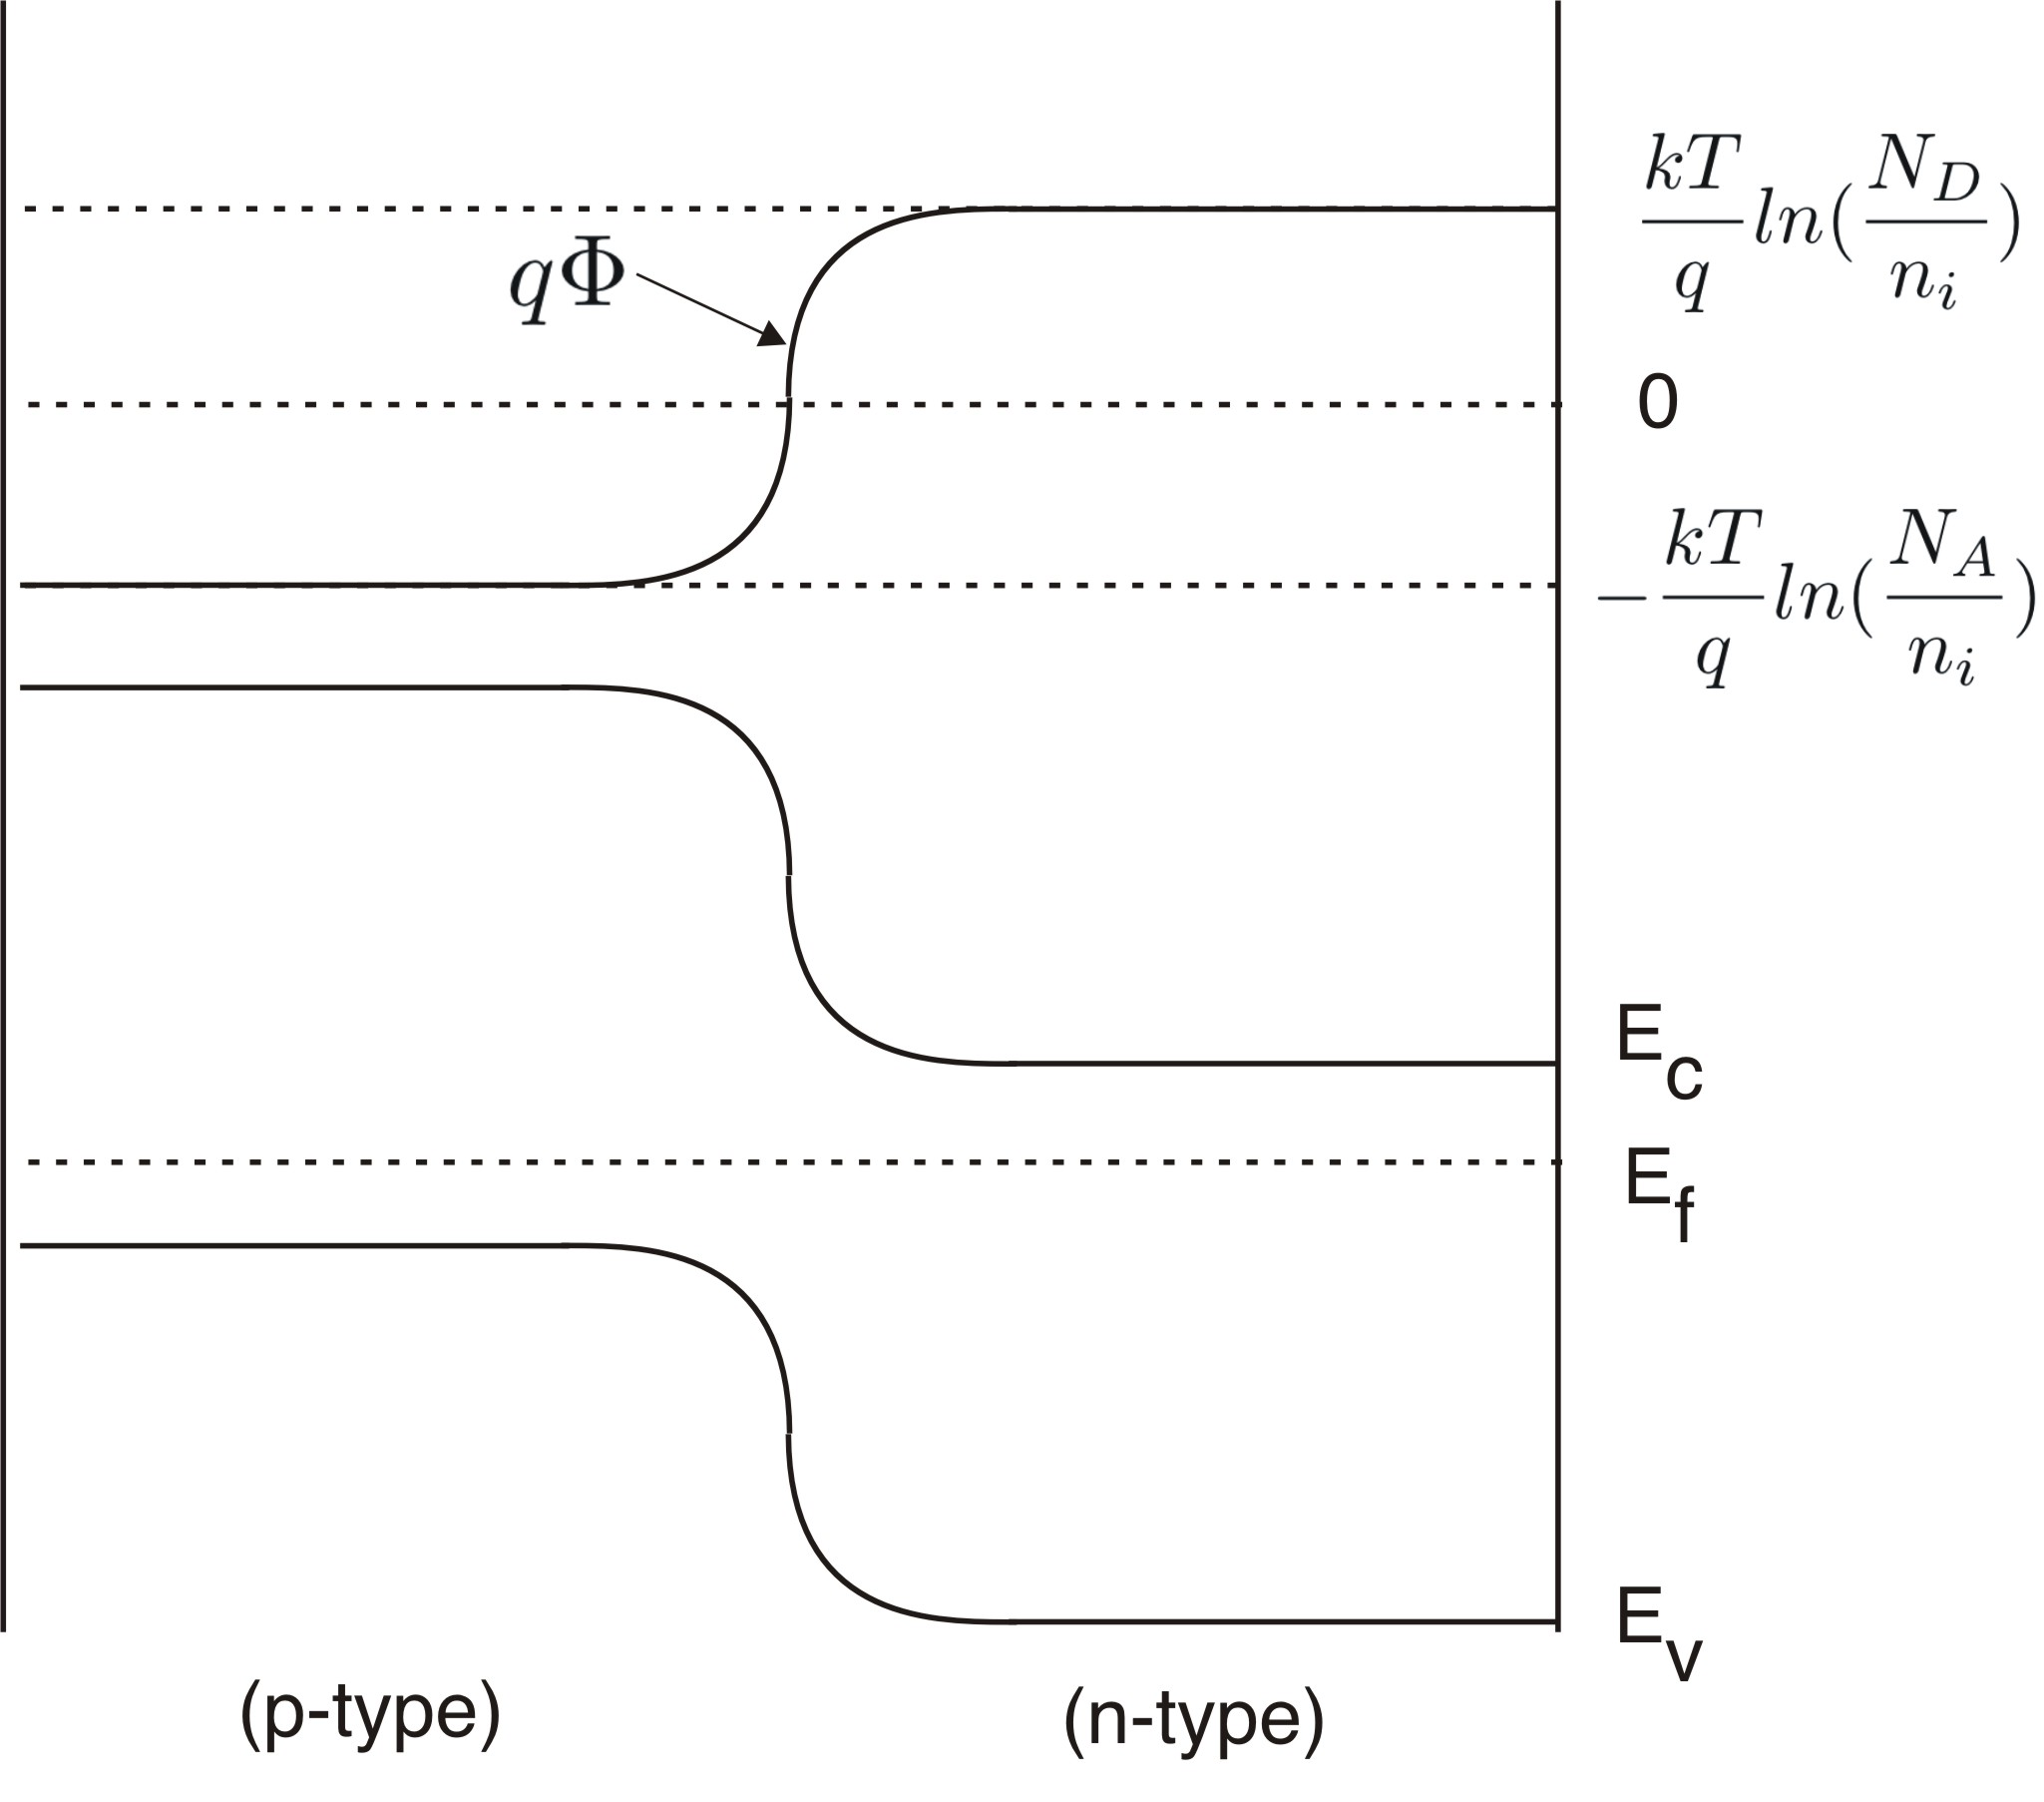
\includegraphics[width=4.050in,height= 3.600in]{neutral_contacts}}
  \caption[Neutral Contacts]{Neutral Contacts. \label{figNeutralContact}}
\end{figure}

$V_{bi}$ represents the extent of the energy band bending due to the doping
of a device.  While most of the dramatic changes will happen away from the
contact, near junctions, it is still incorporated into the voltage boundary
condition to maintain a flat potential near the contacts.  
Figure~\ref{figNeutralContact} shows the energy band variation across a PN
junction, and the corresponding electrostatic potential.  This variation is
due to the internal physics of the device, and needs to be there even in
the event of zero applied voltage.  This is partially enforced by the
solution to Poisson's equation, and also by the application of
equation~\ref{vbc_equ1}.

% Schottky contact figure, P-type

\subsubsection{Schottky Contacts}
In the case of a metal-semiconductor contact, it is necessary to add the
workfunction difference, $\Phi_{ms}$, to the potential in the
semiconductor~\cite{streetman}.  $\Phi_{m}$ is a constant for a given metal, and $\Phi_{s}$
is a function of the doping in the semiconductor.  The workfunction
potential, $\Phi$, when multiplied by q, is the difference between the
Fermi level and vacuum in the material.  In essence, the workfunction
difference represents the distance between the Fermi level in the metal and
the Fermi level in the semiconductor when considering the individual band
structures.

% Schottky contact figure, N-type
\begin{figure}[ht]
  \centering
  \scalebox{1.0}
  {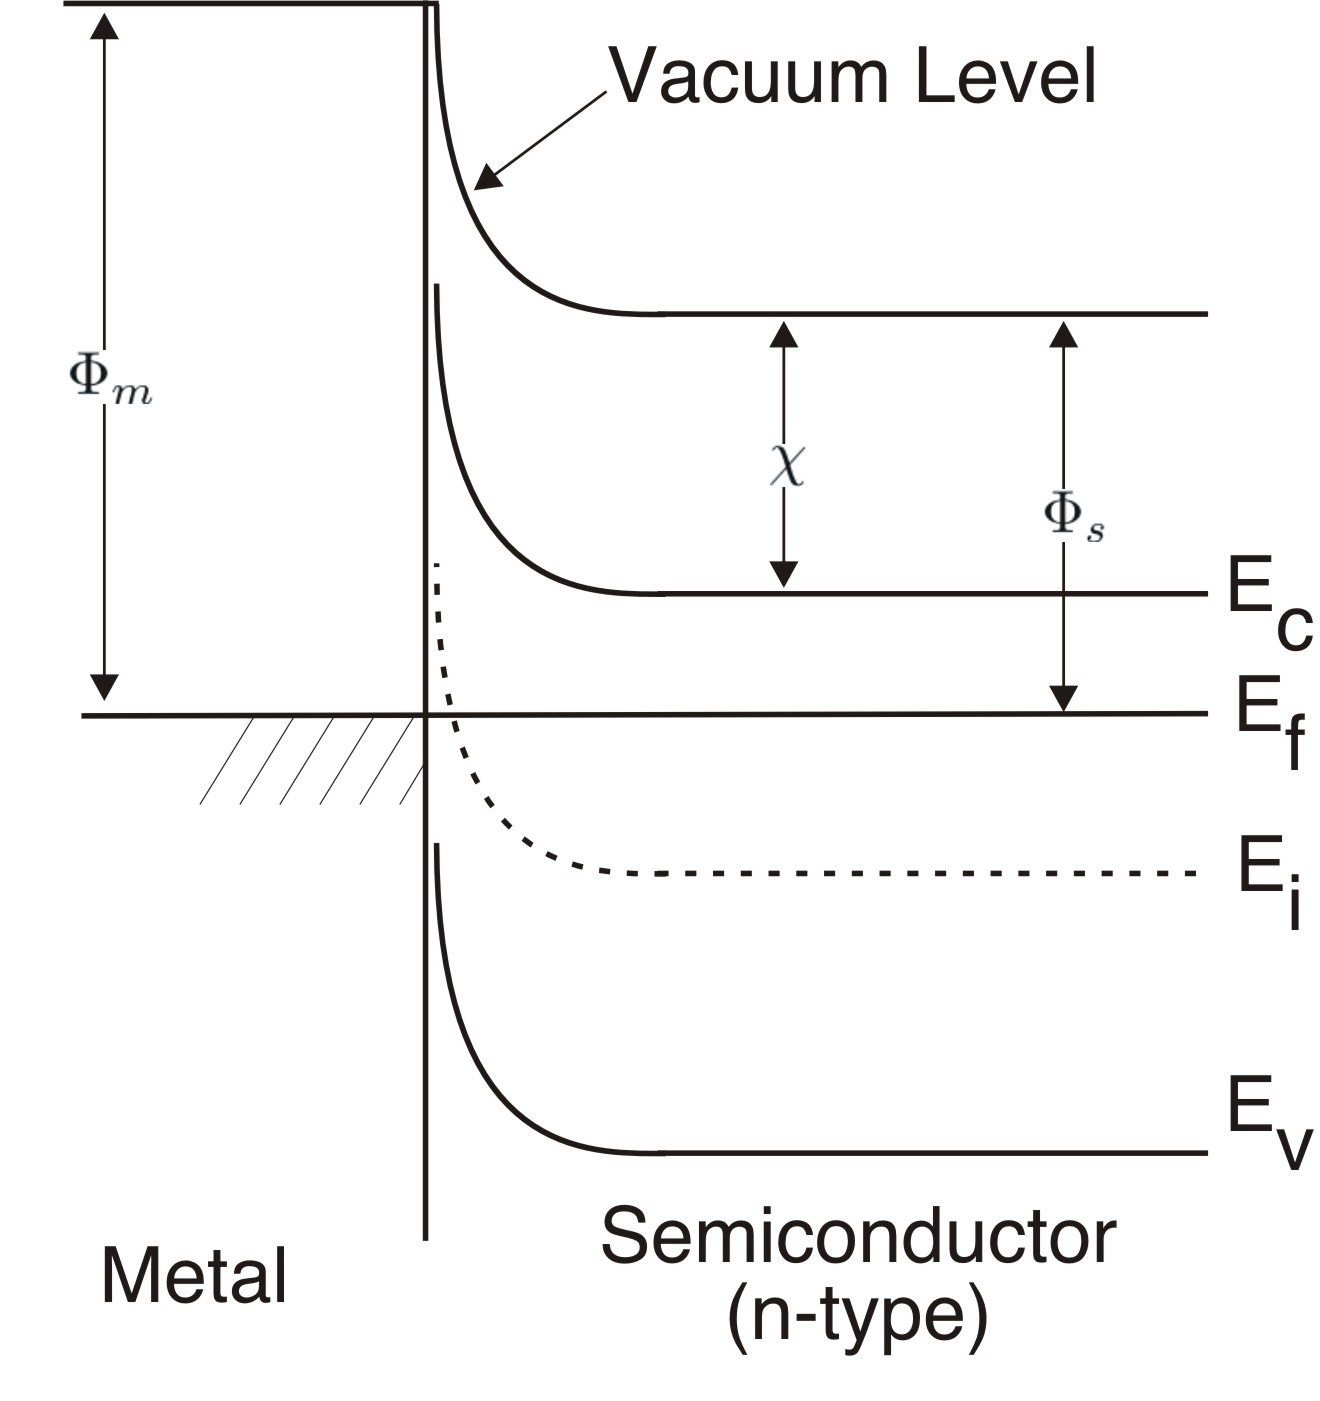
\includegraphics[width=3.300in,height= 3.500in]{schottky_bands}}
  \caption[Schottky Contact, N-type]{Schottky Contact, N-type. 
   \label{figSchottkyContactN}}
\end{figure}

% Schottky contact figure, P-type
\begin{figure}[ht]
  \centering
  \scalebox{1.0}
  {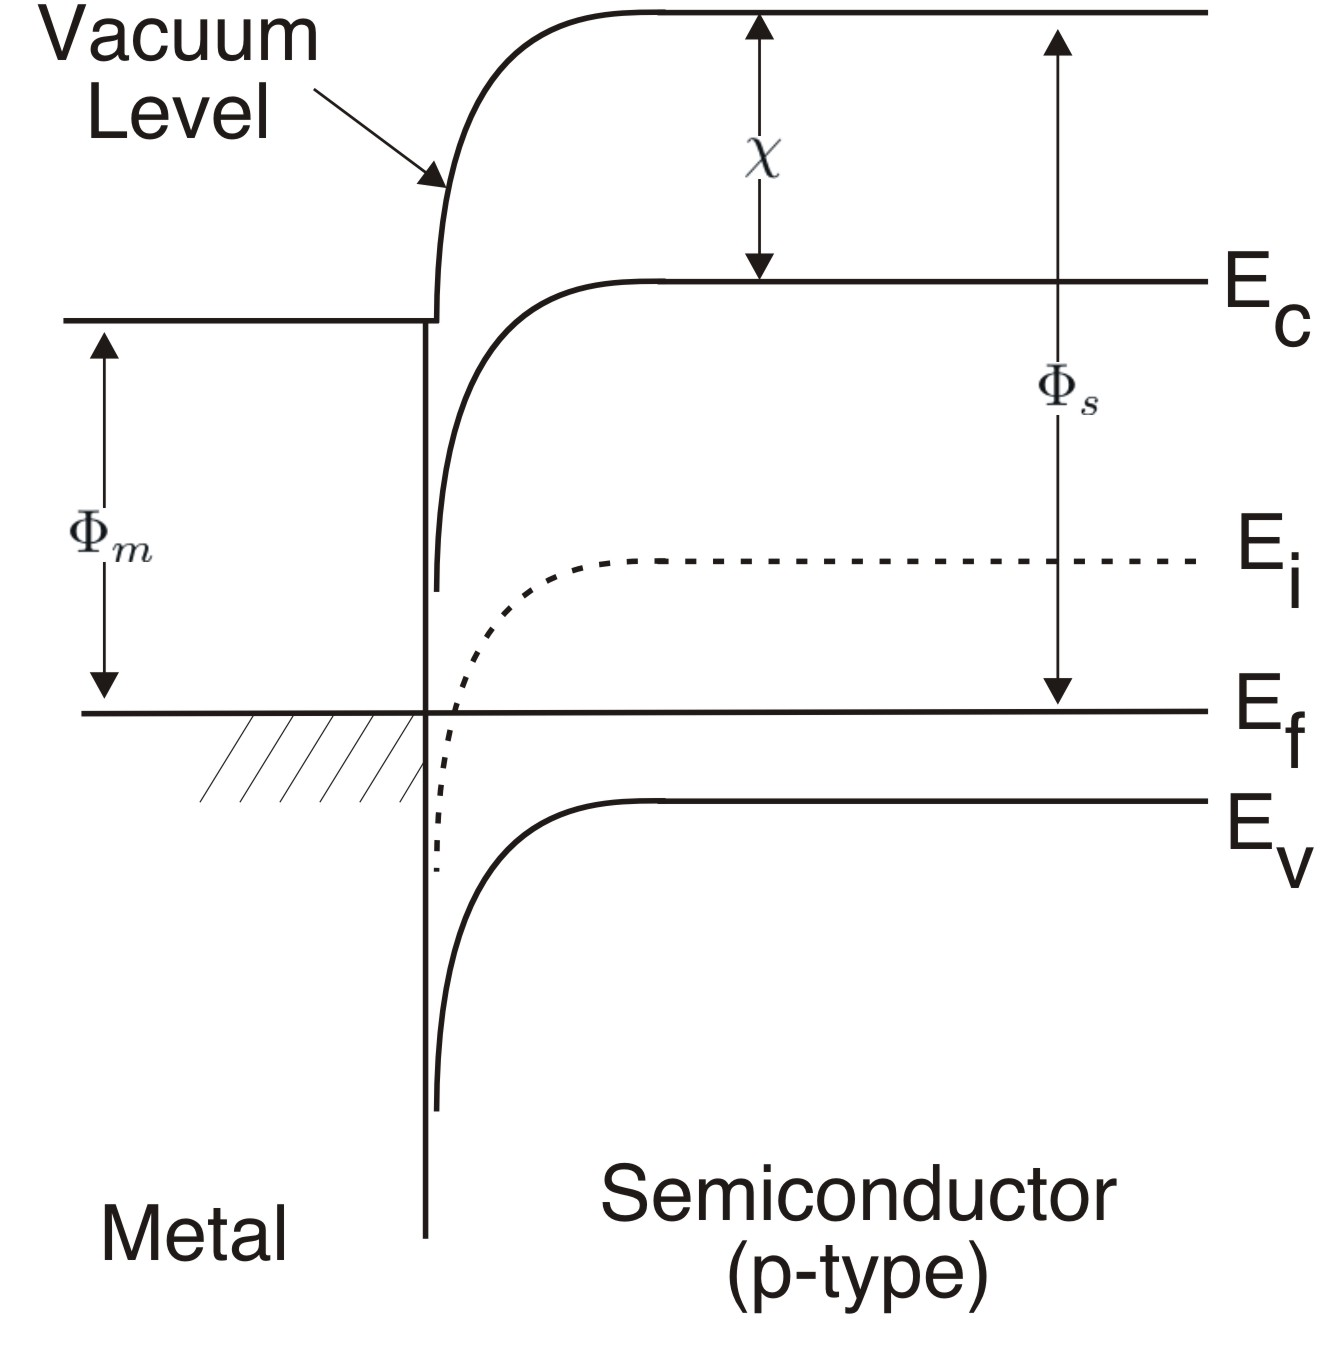
\includegraphics[width=3.300in,height= 3.400in]{schottky_bands_p}}
  \caption[Schottky Contact, P-type]{Schottky Contact, P-type. 
   \label{figSchottkyContactP}}
  
\end{figure}


In the case of an n-type semiconductor, the semiconductor workfunction can
be represented as

\begin{equation}
  \Phi_{s} = \chi + (E_{C}- E_{FS})/q
\end{equation}

where $\chi$ is the electron affinity in the semiconductor and q$\chi$ is the
distance between the conduction band and vacuum in the semiconductor.
$E_C$ is the conduction band energy and $E_{FS}$ is the Fermi level of the
semiconductor.  Rewriting this expression in terms of the doping 
concentration, it becomes

\begin{equation}
  \Phi_{s} = \chi + E_{g}/2 - V_{t}ln(\frac{N_{d}}{n_{i}})
\end{equation}

In the case of a p-type semiconductor, the semiconductor workfunction can
be represented as

\begin{equation}
  \Phi_{s} = \chi + E_{g}/2 + (E_{i}- E_{FS})/q
\end{equation}

where $E_{i}$ is the intrinsic value of the Fermi level, and can be
approximated as the halfway point between the conduction band ($E_{C}$) and the
valance band ($E_{V}$).
Rewriting this expression in terms of the doping concentration

\begin{equation}
  \Phi_{s} = \chi + E_{g}/2 + V_{t}ln(\frac{N_{a}}{n_{i}})
\end{equation}

For the TCAD devices in \Xyce{}, for a node at a metal-semiconductor
contact, the quantity $\Phi_{m} - \Phi_{s}$ is added to the potential at
the node to account for the metal-semiconductor barrier.  The current 
values of metal workfunctions used in \Xyce{} are given in
Table~\ref{workFuncTable}.  The values for electron affinity are given in
Table~\ref{elecAffinTable}.  
The boundary condition for a metal electrode in \Xyce{} is given by

\begin{equation}
 V_{bc} = V_{ckt} + V_{bi} + \Phi_{ms}
\end{equation}

where $V_{ckt}$ is the potential applied by the circuit to the electrode
and $V_{bi}$ is the "built-in" potential of the semiconductor, a
function of the semiconductor doping.

\newpage
\LTXtable{\textwidth}{workfuncTbl.tex}
\LTXtable{\textwidth}{elecAffinTbl.tex}
\newpage

\subsubsection{Metal-Oxide-Semiconductor Contacts}

To date in \Xyce{}, only semiconductor material is included in the PDE
solution domain.  Metals and oxide materials are only included
through boundary conditions.  This is an adequate approach for a lot of
problems.  For some problems (such as modeling of low-dose radiation
effects) modeling the oxide in more detail, as a PDE, will become necessary.
However, since oxides are usually very thin, compared with the
semiconductor domain, meshing both materials as part of the same simulation
is difficult.  Therefore, incorporating the effects of a gate oxide as part
of the gate boundary condition is a reasonable approach.

In the case of a contact to a metal-oxide-semiconductor structure, the
separation of the Fermi energies in the metal and the semiconductor at
equilibrium is due to two effects:  the workfunction difference between the
metal and the semiconductor, and the effective interface charge.  These two
effects cause the bands to bend at the surface in equilibrium.  The
flatband voltage is the sum of these two terms~\cite{streetman}:

\begin{equation}
  V_{FB} = \Phi_{ms} - \frac{Q_{i}}{C_{i}}
\end{equation}

where $\Phi_{ms}$ is the metal-semiconductor workfunction difference,
$Q_{i}$ is the value of interface charge (in $C/cm^{2}$), and $C_{i}$ is the
oxide capacitance per unit area, which is given by

\begin{equation}
  C_{i} = \frac{\epsilon_{ox} \epsilon_{0}}{x_{o}}
\end{equation}

The voltage $V_{FB}$ is the amount of bias which, when applied to the gate,
causes the electron energy bands to be flat.  This is the potential
that is added to a boundary node in \Xyce{} to account for a metal-oxide-semiconductor
barrier.  The overall boundary condition for a contact to a
metal-oxide-semiconductor structure is given by

\begin{equation}
  V_{bc} = V_{ckt} + V_{bi} + \Phi_{ms} - Q_{i}/C_{i}
\end{equation}

where $V_{ckt}$ is the potential applied by the circuit and $V_{bi}$ is the
"built-in" potential of the semiconductor.

\subsubsection{NMOS Device}

The default NMOS device used in \Xyce{} has a substrate doping
concentration of $1.0 \times 10^{16}/cm^{3}$ and an oxide thickness of $1.0
\times 10^{-6}cm$.  Since the ideal threshold voltage $V_{T}$ is given by

\begin{equation}
  V_{T} = 2 \phi_{F} + \frac{\epsilon_{s}}{\epsilon_{ox}} x_{o} 
\sqrt{\frac{2qN_{A}\phi_{F}}{\epsilon_{s}\epsilon_{0}}}
\end{equation}

$V_{T}$ is equal to 0.892 V. for this device.  Note that 
\begin{equation}
  \phi_{F} = \frac{1}{q}[E_{i}(bulk) - E_{F}] = \frac{kT}{q}
  ln(\frac{N_{A}}{n_{i}})
\end{equation}

for a p-type semiconductor substrate and

\begin{equation}
 \phi_{F} = - \frac{kT}{q} ln(\frac{N_{D}}{n_{i}})
\end{equation}

for an n-type substrate.
%%

%%% Local Variables:
%%% mode: latex
%%% End:

% END of Xyce_RG_PDE.tex ************

